\newpage
\appendix

\hypertarget{annexe}{%
\section{Annexe}\label{annexe}}

\hypertarget{appendix:representationGlobal}{%
\subsection{\texorpdfstring{Représentation de l'application \emph{bac à
sable}}{Représentation de l'application bac à sable}}\label{appendix:representationGlobal}}

\hypertarget{firework}{%
\begin{figure}
\centering
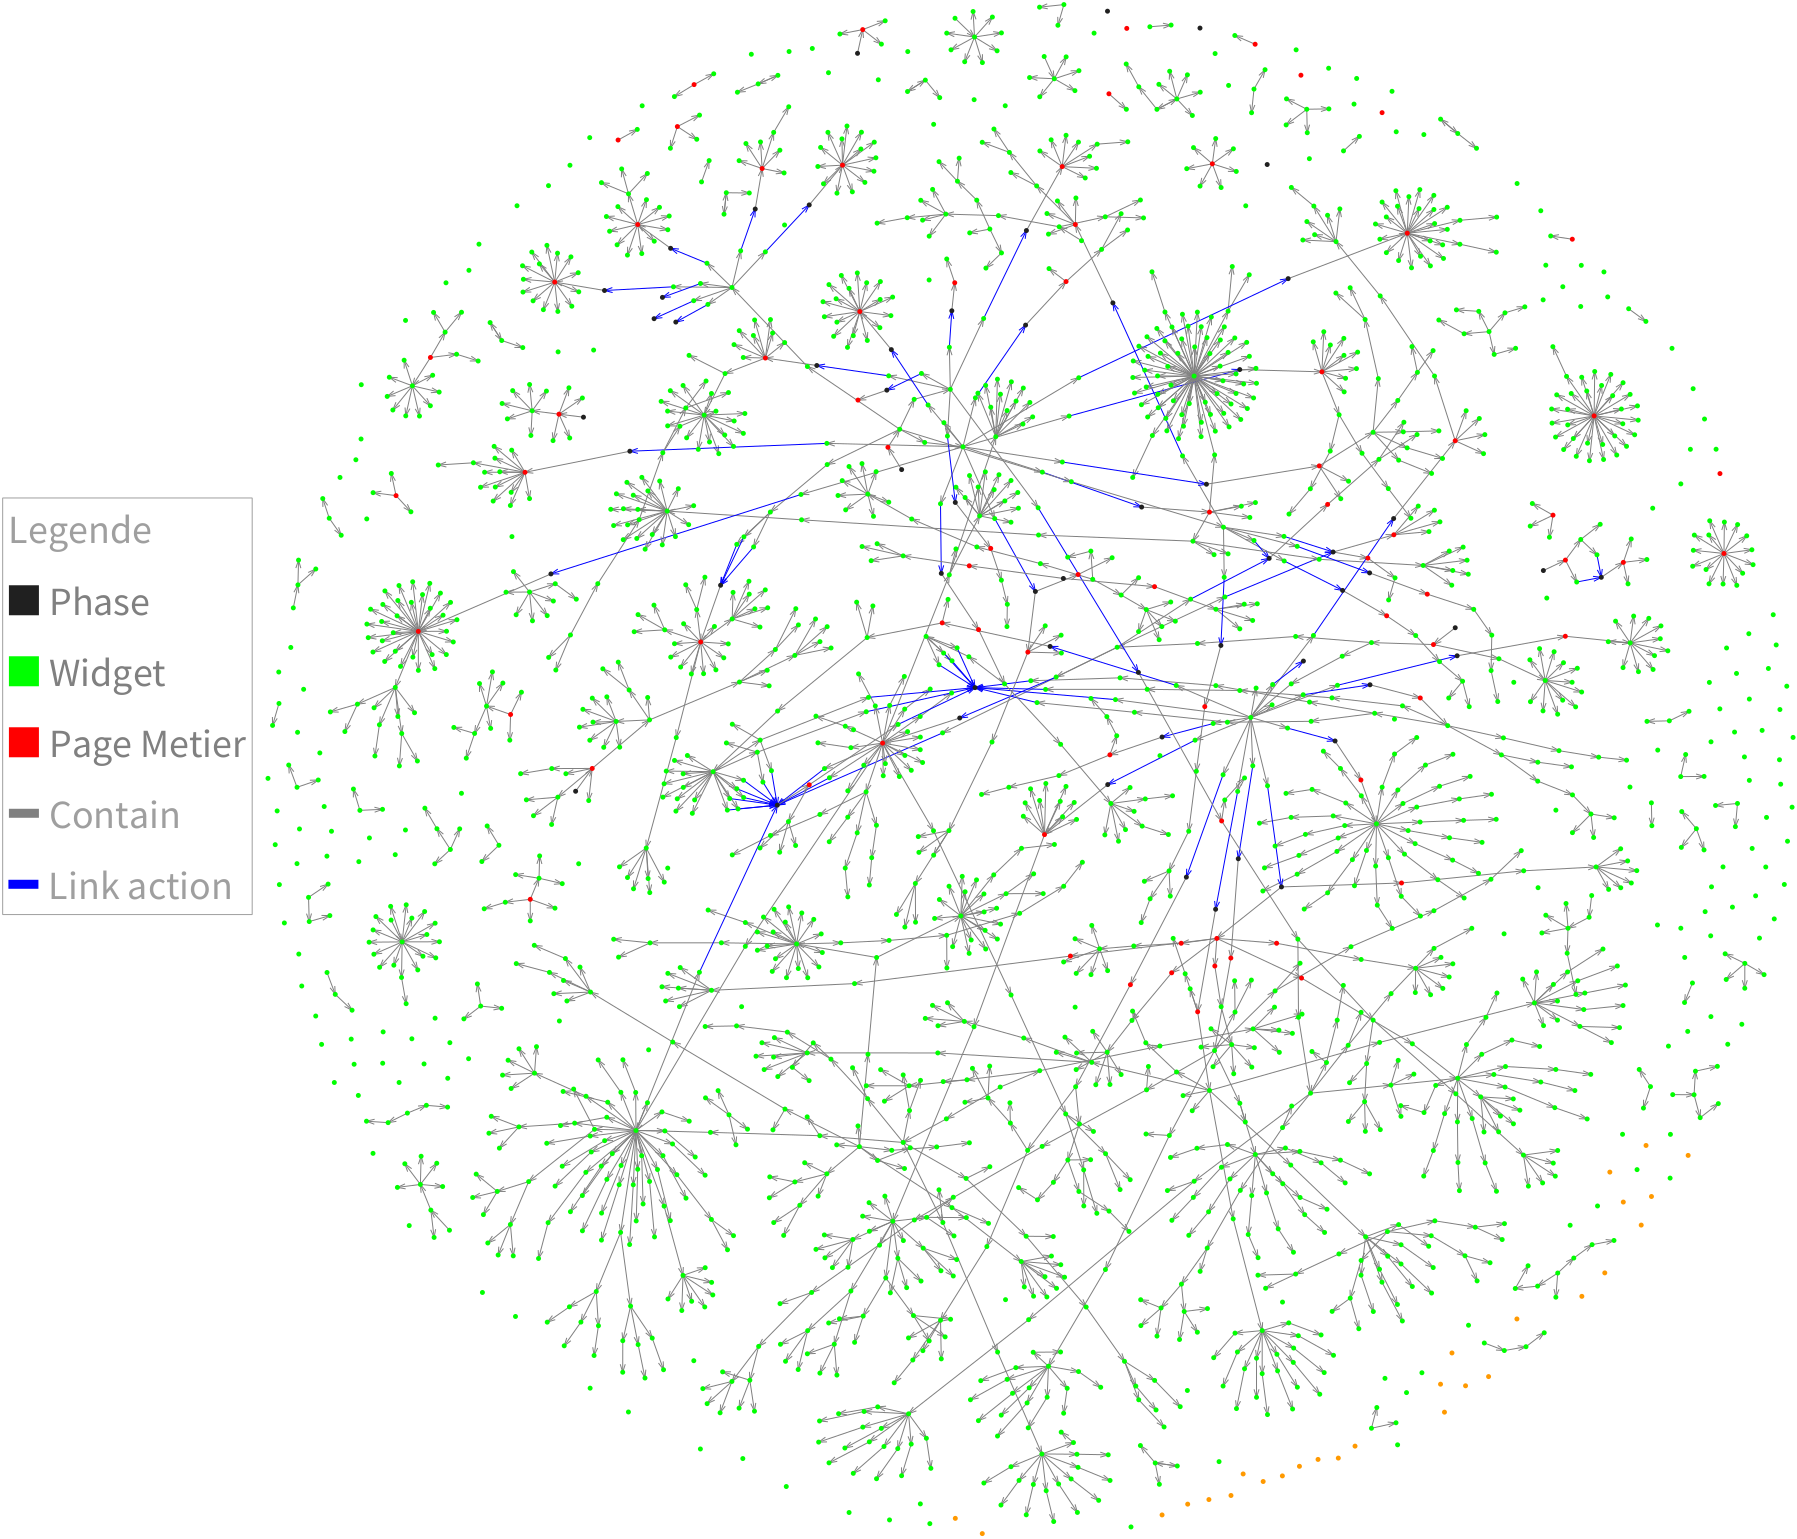
\includegraphics{figures/firework.png}
\caption{Représentation de l'application \emph{bac à sable} dans sa
globalité}\label{firework}
\end{figure}
}

\newpage

\hypertarget{cv}{%
\subsection{CV}\label{cv}}

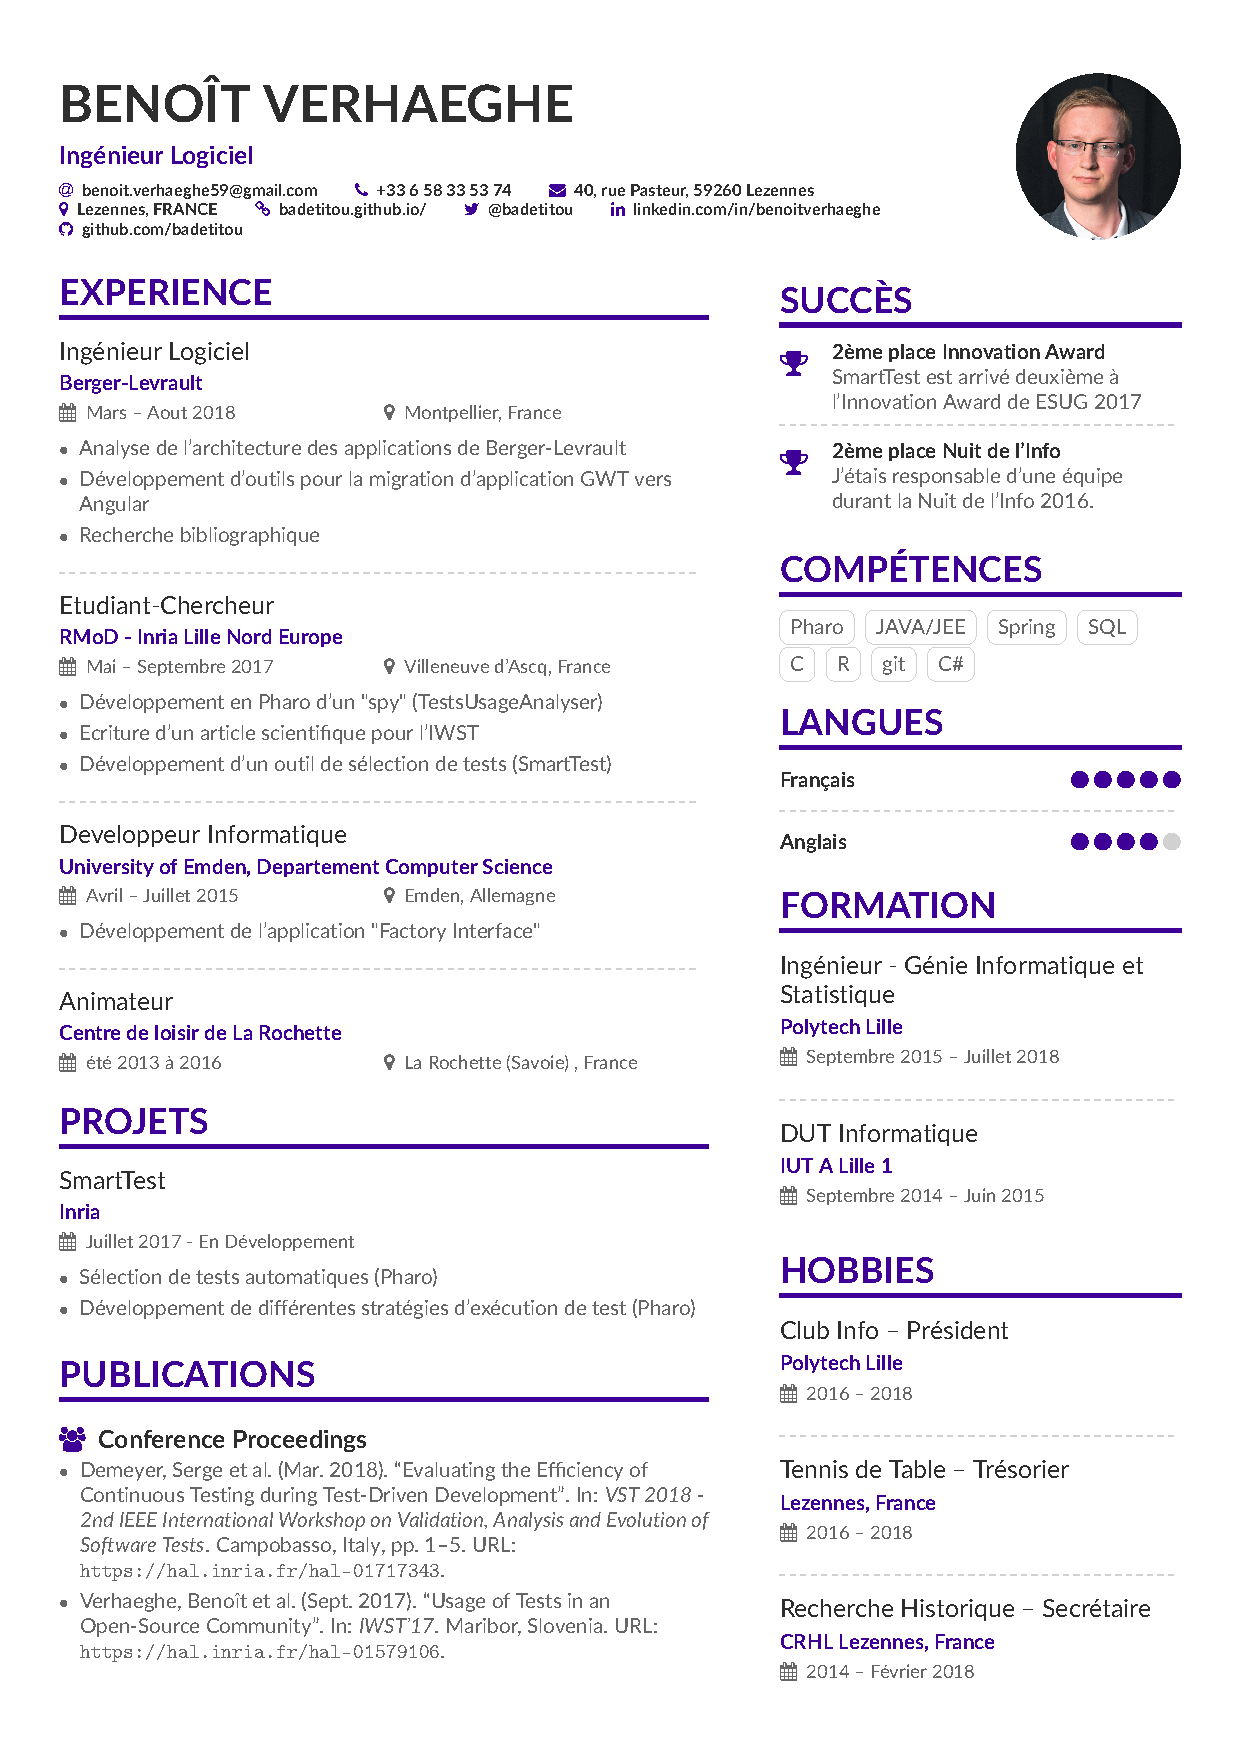
\includegraphics{cv/cv.pdf} \newpage

\hypertarget{ruxe9sumuxe9}{%
\section{Résumé}\label{ruxe9sumuxe9}}

\hypertarget{franuxe7ais}{%
\subsection{Français}\label{franuxe7ais}}

Berger-Levrault est une entreprise majeure dans le monde de l'édition de
logiciel. Dans le cadre de l'évolution de ses applications, elle
souhaite changer le langage d'implémentation de ces derniers. Pour cela,
un travail préliminaire a été mené en Projet de Fin d'Études (PFE) où
l'on a étudié une application de démonstration (\emph{``bac à sable''})
qui reprend les principes d'organisation des applications de
Berger-Levrault. Le but de ce stage était de vérifier que les résultats
de l'étude préalable réalisée durant le PFE peut être appliqué grandeur
nature sur des applications en production de Berger-Levrault et définir
et implémenter une stratégie pour effectuer la migration des
applications. Lors de ce projet, nous avons notamment

\begin{itemize}
\tightlist
\item
  Modélisé des interfaces graphiques d'applications client de
  Berger-Levrault. Le but de cette modélisation est de fournir le
  maximum d'information sur les écrans de l'application pour permettre
  une réimplémentation (semi-)automatique dans un autre langage ;
\item
  Extrait automatiquement des composants des différents écrans de
  l'application ;
\item
  Extrait une carte de navigation entre ces écrans (quel écran permet de
  passer à quel autre écran) ;
\item
  Définit une stratégie, passant par l'utilisation de modèles, pour
  effectuer la migration d'une application disposant d'une interface
  graphique ;
\item
  Réalisé un état de l'art sur le domaine de la migration d'application
  ;
\item
  Migré l'application \emph{bac à sable} de GWT vers Angular.
\end{itemize}

\hypertarget{english}{%
\subsection{English}\label{english}}

Berger-Levrault is a major IT company. As part of the evolution of its
applications, the company needs to switch the application implementation
of its software from GWT to Angular. For this purpose, preliminary work
has been carried out in the End of Studies Project (PFE), where a
\emph{``sandbox''} demonstration application has been studied, which
incorporates the main components of Berger-Levrault's applications. The
purpose of this internship was to verify that the results of the
pre-study carried out during the PFE can be applied to Berger-Levrault
production applications and to define and implement a strategy to
perform the migration of the applications. During this project, we have
in particular

\begin{itemize}
\tightlist
\item
  Modeled Berger-Levrault client application graphical user interfaces.
  The purpose of this modeling is to provide the maximum of information
  on the screens of the application to allow a reimplementation (semi-)
  automatic in another language;
\item
  Automatically extracts components from different screens of the
  application;
\item
  Extract navigation map between these screens (which screen makes it
  possible to switch to which other screen);
\item
  Define a strategy, through the use of templates, to migrate an
  application with a graphical interface;
\item
  Realized a state of the art in the field of application migration;
\item
  Migrated the \emph{``sandbox''} application from GWT to Angular.
\end{itemize}
